%\documentclass[11pt,twoside,lineno]{GSA_format}
\documentclass[11pt,twoside, onecolumn]{GSA_format}
% Use the documentclass option 'lineno' to view line numbers
\usepackage[normalem]{ulem}
\usepackage{float}
\usepackage{amsmath,amssymb}
%\usepackage[textwidth=25cm]{geometry}
\usepackage{siunitx}
\usepackage{arydshln}
\usepackage{graphicx}

\useunder{\uline}{\ul}{}
\articletype{inv} % article type

\newcommand{\bm}[1]{\mbox{\boldmath{$#1$}}}

\newcommand{\beginsupplement}{%
        \setcounter{table}{0}
        \renewcommand{\thetable}{S\arabic{table}}%
        \setcounter{figure}{0}
        \renewcommand{\thefigure}{S\arabic{figure}}%
     }
     
\title{Background selection under evolving recombination rates}

\author[$\ast$]{Tom R. Booker}

\affil[$\ast$]{Department of Zoology, University of British Columbia}

\keywords{Evolutionary genetics, recombination rate, background selection}

\runningtitle{Background selection and recombination rate evolution} % For use in the footer 

\runningauthor{Booker et al}

\begin{abstract}

Background selection (BGS), the effect that purifying selection exerts on evolution at linked sites, is expected to be ubiquitous across eukaryotic genomes. BGS effects reflect the interplay of fitness effects and rates of deleterious mutations with recombination. Leveraging the theory of BGS to analyse patterns of nucleotide diversity has shed light on central issues in evolutionary biology. Fundamental to theoretical models of BGS are recombination rate estimates and an assumption that recombination rates are invariant over time. However, in some lineages recombination rates evolve very rapidly violating this central assumption. Here, we investigate the effect that recombination rate evolution can have on BGS. We show that recombination rate evolution may have localised effects and cause analyses to underestimate the effects genome-wide effects of BGS. Indeed, we find evidence that rapid recombination rate evolution in the recent history of the house mouse may impact inferences of selection in that species.

%It is expected that background selection (BGS), the effect that purifying selection exerts on evolution at linked sites, is ubiquitous across eukaryotic genomes.  The effects of BGS reflect the interplay of the fitness effects and rate of deleterious mutations with the recombination rate.  Leveraging the theory of BGS to analyse patterns of nucleotide diversity in various lineages has shed light on central issues in evolutionary biology. Fundamental to theoretical models of BGS are recombination rate estimates and an assumption that recombination rates are invariant over time. However, in some lineages recombination rates evolve very rapidly violating this central assumption. In this short report, we investigate the effect that recombination rate evolution can have on BGS. We show that recombination rate evolution has an effect on BGS that resembles the effects of population size change. Unlike population size change, however, which may affect the entire genome, recombination rate evolution may have localised effects cause analyses to underestimate the effects genome-wide effects of BGS and demonstrate. Indeed, we find evidence that rapid recombination rate evolution in the recent history of the house mouse may impact inferences of BGS and other forms of selection in that species.

\end{abstract}

\begin{document}

\maketitle

\marginmark

\firstpagefootnote


\correspondingauthoraffiliation{1}{Corresponding author: booker@zoology.ubc.ca}
\vspace{-33pt}% Only used for adjusting extra space in the left column of the first page

\section{Introduction}

Different modes of selection (e.g. positive, purifying and balancing) can all affect variation at linked sites (reviewed in Charlesworth 2008). In the case of purifying selection, the removal of deleterious mutations  can cause linked neutral variants to be lost along with them through a process referred to as background selection (BGS; \citealt{RN132}). Of the mutations that affect fitness, the vast majority are likely deleterious with a comparatively small proportion of beneficial mutations \citep{RN132}. For those reasons, it has been proposed that BGS is likely ubiquitous across eukaryotic genomes and should be incorporated into the null model explaining variation in nucleotide diversity ($\pi$) \citep{Comeron2017-jc, Johri2020}. However, interpreting genome-wide patterns of genetic variability in terms of BGS requires accurate estimates of population genetic parameters, particularly recombination rates.
 

%One effect of BGS is a reduction in genetic diversity for regions of the genome subject to purifying selection. The expected reduction in nucleotide diversity ($\pi$) under BGS is proportional to the ratio of the local deleterious mutation rate and the local recombination rate  \citep{RN132, RN157, RN206}. The first empirical evidence that selection at linked sites of any kind influences genetic variation across the genome came from studies in \textit{Drosophila}. \cite{RN225} measured genetic variability in the \textit{yellow-achaete-scute} regions located at the tip of the X-chromosome in \textit{D. melanogaster}. The \textit{yellow-achaete-scute} regions experience restricted crossing-over and  \cite{RN225} found that they harbour far less genetic variation than had been reported for more highly recombining regions of the genome. Subsequent studies demonstrated a positive correlation between nucleotide diversity and recombination rate genome-wide in \textit{D. melanogaster} \citep{RN114} and similar patterns have been reported in numerous other species \citep{RN117}. 

\vspace{5px}
 
Recombination rates vary across the genome. For example, in mice, the local recombination rate ($r$) can vary substantially across a chromosome \cite{RN263}. The locations of actual recombination events in mice are typically restricted to narrow windows of the genome (on the order of 1-5 Kbp), referred to as hotspots \citep{RN263}. The locations of recombination hotspots in mice, and many other vertebrates, are determined by the binding of a protein encoded by the \textit{PRDM9} gene to specific DNA motifs \citep{RN269, Baker2017}.

\vspace{5px}

Estimates of the local recombination rate ($r$) can be obtained empirically by examining the inheritance of genetic markers through known pedigrees, as in traditional genetic mapping, or by directly comparing an individual's genome to that of its gametes (e.g. \citealt{Sun2019}). Both methods directly observe recombination events over one or fairly small number of generations, and thus provide estimates of $r$ for contemporary populations. Alternatively, estimates of $r$ can be obtained indirectly by analysing linkage disequilibrium across the genome (e.g. \citealt{Spence2019}) and such estimates reflect both recent and ancestral recombination events. The use of empirical or indirect estimates of recombination rate when analysing genome-wide variation in $\pi$ in terms of BGS implicitly assumes that the recombination landscape has not changed over the time in which patterns of diversity have been established. However, temporal variation in the recombination rate may influence our ability to explain population genomic data using BGS as our null model as described by \cite{Comeron2017-jc}.

\vspace{5px}


Recombination rate changes may influence fine-scale patterns of molecular evolution. For example, chromosomal fusions would decrease recombination rates experienced by individual nucleotides, and thus increase the effects of BGS and other processes mediated by recombination. Consistent with this, \cite{Cicconardi2021}  found evidence suggesting that chromosomes that underwent fusions in the ancestors of extant \textit{Heliconius} butterfly species now harbour lower $\pi$ due to reduced recombination rates and presumably greater BGS effects. Following evolution of the recombination rate landscape, there will be a lag period wherein patterns of genetic variability more closely reflect ancestral recombination rates than derived rates. Depending on how recombination rate landscapes evolve, population genomic analysis of lineages that are still within that lag period may be obscured. In this letter, we examine how patterns of neutral genetic variability under BGS respond to evolution of the recombination rate and describe how this may have affected analyses that are used to identify the effects of selection genome wide. 

\section{Results and Discussion}

\subsection{Background selection under evolving recombination rates}
%The analogy is not perfect, because it does not capture the effects of weakly deleterious mutations (BGS Papers). 

A change in the recombination rate will alter the effects of BGS. Under strong purifying selection, BGS reduces coalescence times and resembles a localised reduction in the effective population size ($N_e$). Changes in the recombination rate for a particular genetic region may therefore resemble a localised change in $N_e$. For a neutral site $\nu$, the combined effects of recombination, mutation and purifying selection cause there to be a reduction of $B_{\nu,0}$ to coalescence times. At time $T_0$ in the past (in $2N_e$ generations), the population underwent an instantaneous change in the recombination rate so $\nu$ now experiences a BGS effect of $B_{\nu,1}$. Equation 1a from \cite{Johri2020} describes coalescence times after instantaneous population size change. We modified their expression, incorporating the effects of BGS before and after a change in the recombination rate:

\begin{equation}
B_{\nu,\Delta r} = B_{\nu,1} ( 1 + (\frac{B_{\nu,0}}{B_{\nu,1}} - 1)e^{-T_0})
\label{BGS_rec}
\end{equation}
\noindent
Note that \cite{Pool2007} provided similar expressions to those given by \cite{Johri2020}.

\vspace{5px}
 

We modelled deleterious mutations occurring in a single functional element and examined $\pi$ for neutral mutations in and around this region after an instantaeous change in the recombination rate (Figure \ref{fig:BGS_over_time_fixed_s} and \ref{fig:BGS_over_time_multiPanel}). Up to $2N_e$ generations after a change in the recombination rate, $\pi$ more closely resembles the expectation under the ancestral recombination rate than it does the derived rate (Figure \ref{fig:BGS_over_time_fixed_s}). After around $4N_e$ generations, coalescence times closely reflect those expected under BGS given the derived recombination rate, as measured by $\pi$ (Figure \ref{fig:BGS_over_time_fixed_s}). The results in Figure \ref{fig:BGS_over_time_fixed_s} were obtained assuming deleterious mutations with constant effect, a distribution of fitness effects for harmful mutations leads to similar results (Figure S2). When deleterious mutations have only mild effects, Equation \ref{BGS_rec} does not fit the observed data particularly well (Figure SX - Add this?) because in such cases BGS does not resemble a simple reduction in $N_e$ \citep{Good2014, Cvijovic2018}. 


\begin{figure}[H]
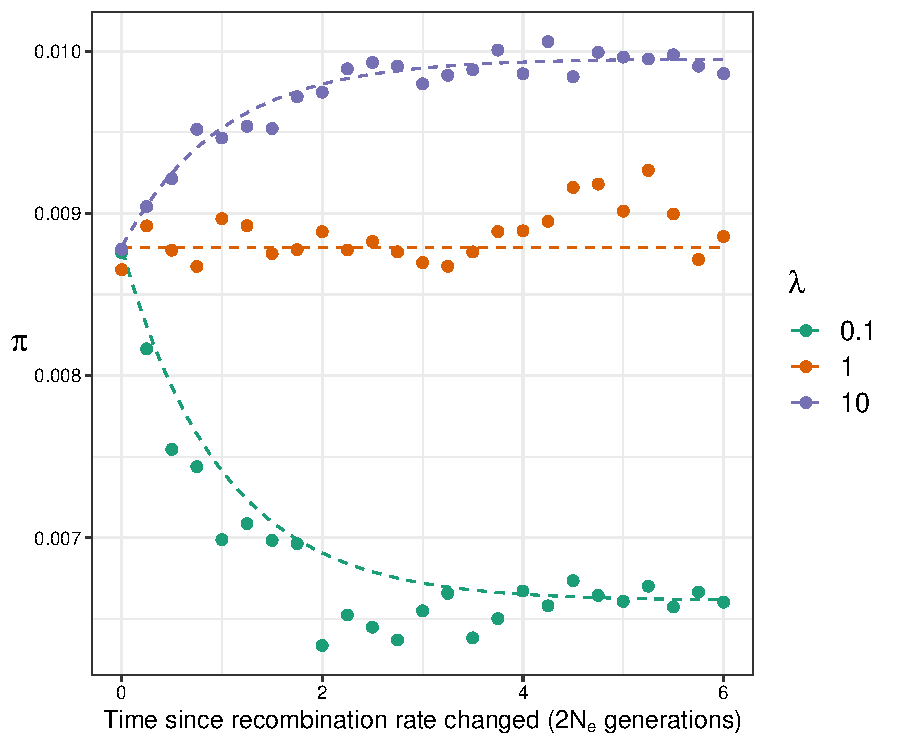
\includegraphics[width=0.5\textwidth]{../TheoreticalExpectation/B_over_time_fixed_s_plot_singlePanel}
\caption{Nucleotide diversity over time after recombination rates change by a factor $\lambda$. The dashed lines were calculated using Equation \ref{BGS_rec}, points indicate the mean from 100 replicate simulations.}
\label{fig:BGS_over_time_fixed_s}
\end{figure}

\subsection{Patterns of genetic variation after evolution of the recombination landscape}


Consider a population that has recently undergone shifts in the recombination rate landscape (i.e. less than $2N_e$ generations ago). Estimates of $r$ from such a population would likely reflect contemporary recombination rates regardless of how they were obtained. Empirical estimates of $r$ always reflect contemporary rates and indirect estimates (i.e. obtained from patterns of LD) can reflect contemporary recombination rates within 0.5$N_e$ generations of a change (Figure \ref{fig:recombinationRateEstimates}). Depending on the extent and nature of recombination rate evolution, population genomic analyses that compare features of genetic variability to estimates of $r$ may be obscured. 

\vspace{5px}

To demonstrate how population genomic analyses may be affected by changes in $r$, we simulated two scenarios of BGS under evolving recombination rates. In the first, the broadscale landscape of $r$ is rearranged, approximating a burst of karyotype evolution (Figure \ref{fig:recombinationRateMaps}A). In the second, the locations of recombination hotspots are shifted, as if a new PRDM9 allele had fixed in a population (Figure \ref{fig:recombinationRateMaps}B). In both scenarios, deleterious mutations occur across the genome generating widespread BGS such that at equilibrium there is a positive correlation between $\pi$ and $r$ (Figure \ref{fig:correlationOverTime}).

\vspace{5px}

A positive correlation between $\pi$ and $r$ is the hallmark signature of widespread selection across a genome \citep{RN117}, but evolution of the recombination rate may obscure such a pattern. In both of the scenarios we simulated, during the lag period after recombination rate change the correlation between $\pi$ and $r$ would be misleading (Figure \ref{fig:correlationOverTime}). In both cases, a strongly significant positive correlation re-establishes after about $2N_e$ generations (Figure \ref{fig:correlationOverTime}). When recombination maps evolved by the movement of hotspots, the scale at which $\pi$ and $r$ are estimated determined whether a positive correlation between $\pi$ and $r$ was found (Figure \ref{fig:correlationOverTime}). Of course there are reasons why species may not exhibit a positive correlation between $\pi$ and $r$ \citep{RN117} that have nothing to do with recombination rate evolution. For example wild and domesticated rice (\textit{Oryza spp.}) exhibit negative correlations between $\pi$ and $r$, but in those species there is a strong positive correlation between the density of functional sites (i.e. sites subject to purifying selection) and the recombination rate (Flowers et al 2011).

\vspace{5px}

\begin{figure}[H]
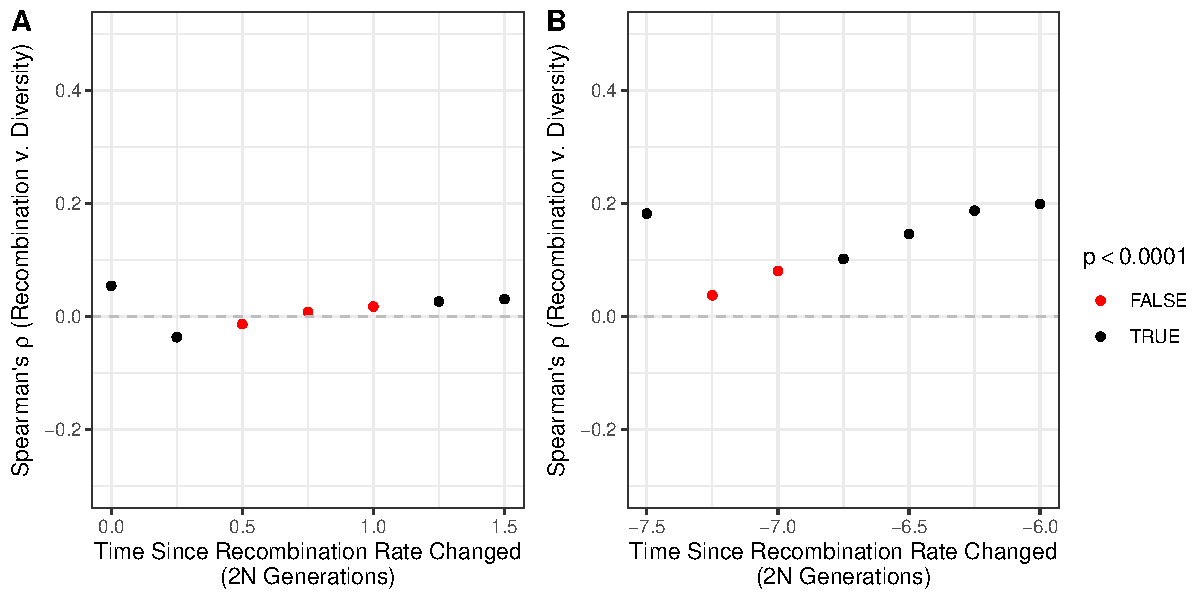
\includegraphics[ width = \textwidth]{../Plots/pi_r_correlationOverTime_bothMaps.pdf}
\caption{Spearman's correlation between nucleotide diversity ($\pi$) and recombination rate ($r$) over time after recombination rates evolve. Results are shown for 100 Kbp analysis windows. } 
\label{fig:correlationOverTime}
\end{figure}


\subsection{Rapid recombination rate evolution in house mice}

Recombination rate landscapes can evolve very rapidly. For example, due to the requirement of at least one cross-over per chromosome per meiosis in mammals, changes in chromosome length induce changes in $r$ and thus karyotype evolution likely influences the recombination rate. The lineage leading to \textit{Mus musculus} (2\textit{n}=40) has experienced large chromosomal rearrangements since it shared a common ancestor with \textit{Mus pahari} (2\textit{n}=48) 3-5 million years ago \citep{Thybert2018}. Moreover, there are differences in $r$ among populations of \textit{Mus musculus domesticus} that harbour different karyotypes \citep{Vara2021}. Chromosomal fusions can exhibit meiotic drive \citep{Chmatal2014} so new karyotypes may spread to fixation very rapidly. There is also evidence that \textit{PRDM9}, the gene that encodes the protein that dictates the locations of recombination events, has undergone recurrent bouts of positive selection in mice \citep{RN329} and natural populations of \textit{M. musculus spp.} posses various \textit{PRDM9} alleles corresponding to different suites of recombination hotspots \citep{RN249}. Overall, there is clear evidence from mice that recombination rates can evolve rapidly at broad and fine scales. 

\vspace{5px}

It is plausible that rapid evolution of recombination rates in \textit{Mus musculus} has influenced our ability to identify the effects of selection across the species' genome. \cite{Kartje2020} recently demonstrated that natural populations of \textit{M. m. domesticus} exhibit a very weak correlation between $\pi$ and $r$ and concluded that there was fairly limited effects of BGS genome-wide. This is somewhat unexpected, however, because wild mice are thought to have large effective population sizes (Leffler et al 2012) and genome-wide evidence for selection is thought to be apparent in species with large $N_e$ \citep{RN117}. If the burst of karyotype evolution that occurred over the last few million years in the ancestors of house mice affected recombination rates, then mouse populations may be within the lag period described by Equation \ref{BGS_rec}. If patterns of genetic diversity in mice are still adjusting to changes in the recombination rate, we might see a stronger correlation between $\pi$ and $r$ in genomic regions that have not undergone dramatic changes in the recombination rate. 

\vspace{5px}

Using an alignment of genomes from closely related species, \cite{Thybert2018} identified chromosomes in the \textit{M. musculus} genome that have or have not undergone dramatic rearrangements in the last 5 million years. We re-analysed data from \cite{Kartje2020} and found that the correlation between $\pi$ and $r$ is stronger and more significant on chromosomes that have not undergone rearrangements in the last 3-5 million years (Table \ref{Table1}) for \textit{M. m. domesticus} individuals from France and Germany. This pattern holds when looking at analysis windows of 5 Kbp and 1 Mbp (Table \ref{Table1}). \textit{M. m. domesticus} colonised Gough Island in the 19th century and experienced a severe population bottleneck (Grey et al 2014), which may have further obscured patterns of variability. 

\vspace{5px}

Evolution of the recombination rate is just one of a large number of possible reasons why one might not be able to adequately identify the effects of BGS (or natural selection more broadly) from population genomic data \citep{Comeron2017-jc}. Our re-analysis suggests that mice are still within the lag period after evolution of the recombination rate, such that $\pi$ in \textit{M. m. domesticus} does not fully reflect contemporary recombination rates in \textit{Mus musculus}. In contrast, the ancestors of \textit{Heliconius} butterflies also underwent large-scale karyotype evolution, but gross patterns of $\pi$ versus chromosome length in those species suggest that patterns of variation have largely re-equilibrated after changes in $r$ \citep{Cicconardi2021}. In some lineages, recombination rate evolution may be very slow. Birds, for example, have highly conserved karyotypes and in some cases highly conserved recombination landscapes (Damas et al 2018; Singhal et al 2017). 

\vspace{5px}

This short paper should add to the growing appreciation of recombination as an evolutionary labile trait. As pointed out by \cite{Comeron2017-jc} and Smukowski Heil et al (2015), information on recombination rates in outgroup species is an important covariate in 
when performing population genomic analyses. Throughout this short paper, we have referred to recombination as a fixed trait that is not variable among individuals, but that is certainly not the case. Heritable variation in recombination rates have been reported in several species (reviewed in Stapley et al 2017).



\begin{table*}[t]
\
\resizebox{\textwidth}{!}{\begin{tabular}{cc|
           *{2}{S[round-mode = figures,
            round-precision = 3]}|
                 *{2}{S[round-mode = figures,
            round-precision = 3]}|
                 *{2}{S[round-mode = figures,
            round-precision = 3]}}
                 \hline
 & & \multicolumn{2}{c}{Whole Genome} & \multicolumn{2}{c}{Conserved Chromosomes}& \multicolumn{2}{c}{Non-Conserved Chromosomes}\\
 {Window} & {Population} &  {Spearman`s $\rho$} & {$p$-value} &{Spearman`s $\rho$} & {$p$-value} & {Spearman`s $\rho$} & {$p$-value}\\ 
  \hline
5Kbp& Gough Island & 0.00766946556467726 & \num{4.28487483542177e-05} & 0.00879560871962056 & 0.0102132179985377 & 0.00485568404015206 & 0.0301693742321603 \\ 
  5Kbp & France & 0.00408044307052427 & 0.0294929095581957 & 0.0402631172537313 & \num{6.10313340830373e-32} & -0.0107049632666829 & \num{1.75806407865671e-06} \\ 
  5Kbp & Germany &  0.00752167382031877 & \num{6.05264156648312e-05} & 0.0151531276721775 & \num{9.6335227129151e-06} & 0.00386135398506519 & 0.0849380013628119 \\ 
  1Mbp & Gough Island &  0.0535515289545324 & 0.00946379855975982 & 0.0588327090738239 & 0.124246200526924 & 0.043697649001863 & 0.0748313470537267 \\ 
  1Mbp & France &  0.0449712235482249 & 0.0293606123894296 & 0.134981255195878 & 0.000400166310010629 & 0.00998569897732337 & 0.684066944892074 \\ 
  1Mbp & Germany &  0.0535221710805316 & 0.00953371381645413 &  0.0774668203290588 & 0.0428305229197646 & 0.0425693100291219 & 0.0828457161038532 \\ 
\hline
\end{tabular}}

\caption{The correlation between nucleotide diversity ($\pi$) and recombination rate for three populations of house mice (\textit{Mus musculus domesticus}) calculated from all autosomes, conserved chromosomes that exhibit no syntenic breaks between \textit{M. musculus} and \textit{M. pahari} and the non-conserved chromosomes as identified by Thybert et al (2018).}
\label{Table1}
\end{table*}







%We have restricted our analysis to what happens when fitness affecting mutations are strictly deleterious and generate BGS. However, other modes of selection and their effects on linked variation may also affect nucleotide diversity. For example, there is evidence that recurrent selective sweeps influence diversity patterns in numerous species \citep{Nam2017, RN323, RN274}. It seems reasonable to expect that recombination rate evolution would also influence inferences about selective sweeps.  


\section{Methods}
\subsection{Model}
Background selection has been modelled as the reduction in effective population size ($N_e$) at a neutral site due to the removal of deleterious variants. The effects of background selection are often expressed as $B = \frac{N_e}{N_0}$, where $N_e$ is the effective population size and $N_0$ is the expected population size under strict neutrality. In a non-recombining genome, $B$ is proportional to the ratio of the deleterious mutation rate to the strength of selection acting on harmful mutations (Charlesworth et al 1993). For a neutral site present on a recombining chromosome, the effects of background selection depend on the density of functional sites (i.e. those that can mutate to generate deleterious alleles), the mutation rate, the strength of selection and the recombination rate (Hudson and Kaplan 1995; Nordborg et al 1996; Nordborg 1997). For a neutral locus $\nu$ linked to $x$ functional sites, the reduction in $N_e$ has been described with the following equation:

\begin{equation}
B_{\nu} = \frac{N_e}{N_0} = exp[ -\sum\limits_x \frac{u_x}{t(1+(1-t)r_{x,v}/t)^2} ]
\label{nordborg}
\end{equation}\noindent
Where $u_x$ is the deleterious mutation rate at functional site $x$, $t$ is the heterozygous fitness effect of a deleterious mutation (i.e. 0.5$s$ in the case of semi-dominance) and $r_{x,\nu}$ is the recombination map distance between the neutral locus and functional site $x$. In the above equation, deleterious mutations have fixed effects, but it is straightforward to incorporate a distribution of fitness effects \citep{RN157}. The above equation holds when selection is sufficiently strong  such that random drift does not overwhelm selection ($N_es > 1$) \citep{Good2014}. \\
 


\subsection{Simulations}

We simulated BGS under recombination rate evolution using two types of simulations in \textit{SLiM} v3.2 \citep{Haller2019-jv}. Diploid populations of $N_e$ = 5,000 individuals were simulated and in all  cases we scaled the parameters by population size to species with large larger $N_e$. \\


The first set of simulations was designed to examine how long it takes for patterns of neutral diversity under BGS to equilibrate after the recombination rate evolves. In these simulations, the genome was 25Kbp long with a 5Kbp functional element in the centre. Mutations occurred in the functional element at rate $\mu = 2.5\times10^{-6}$ and had semi-dominant fitness effects with a fixed selection coefficient of $s = -0.01$. We also simulated cases with varying fitness effects using a gamma distribution with mean ($\bar{s}$) of -0.1 and a shape parameter of 0.1. Recombination occurred at a uniform rate of $r = 2.5\times10^{-6}$ across the chromosome. After 15,000 generations, we simulated an instantaneous change in the recombination rate, multiplying $r$ by $\lambda$, giving $r = \lambda2.5\times10^{-6}$. We simulated cases with $\lambda$ = 0.1, 1.0 and 10.0. Simulated populations were sampled every 500 generations after the recombination rate changed and we performed 200 replicates for each set of parameters tested. Note that these simulations were not designed to be particularly realistic, but to provide clear cut patterns to test the theoretical predictions. \\

The second set of simulations was designed to examine how patterns of $\pi$ versus $r$ varied over time when recombination rates evolved at fine and/or broad scales. For these simulations, we modelled chromosomes that were 10Mbp long. Neutral mutations occurred at random across the length of the sequence at a rate of $5\times10^{-6}$. Deleterious mutations occurred at random across the length of the sequence at a rate of $2\times10^{-8}$ with semi-dominant fitness effects drawn from a gamma distribution with a mean ($\bar{s}$) of -0.1 and a shape parameter of 0.1. The deleterious mutation rate was chosen so that 4\% of the genome was subject to purifying selection. Populations evolved under background selection for 100,000 generations (i.e. $20N_e$ generation). In generation 100,000 there was instantaneous evolution the recombination landscape after which we recorded the tree-sequence of the population every 5,000 generations for . We incorporated two models of recombination rate variation and evolution of the recombination map:
\begin{itemize}

\item[•] We modelled recombination rate evolution at broad scales by rearrangement of the recombination landscape. Recombination rates vary across the genome (Shapley et al 201s8). For example, recombination rates vary by a factor of 3 acros chromomsome 1 in mice. In these simulations, recombination varied from $r=2.08\times10^{-7}$ to $r=6.24\times10^{-7}$. When the recombination landscape evolved, we reversed the order of recombination rates across the genome (Figure \ref{fig:recombinationRateMaps}A).

\item[•] We modelled the evolution the recombiantion map by the movement of hotspots. Recombination occurred at a uniform rate of $r=6\times10^{-8}$ except in 5Kbp hotspots where it occurred at a rate of $r=6\times10^{-6}$. At the beginning of a simulation, a Poisson number of hotspots was sampled with an expectation of 120. Hotspots were placed at random across the simulated chromosome. When the recombination landscape evolved, we resampled the locations of hotspots (Figure \ref{fig:recombinationRateMaps}B).

\end{itemize}

\noindent In both cases, rates were chosen such that the total map length was similar to one that recombined at a constant rate of $4N_er=0.008$, the value reported for wild mice (Booker et al 2017). \\

For all simulations, we used the tree sequence recording option in \textit{SLiM} and neutral mutations were added to the resulting tree-sequences at a rate of $5\times10^{-7}$ using \textit{PySLiM} and \textit{msprime} \citep{Haller2019-za, Kelleher2016-zz}. Nucleotide diversity ($\pi$) was calculated in windows of varying size using sci-kit-allel. We used the program \textit{PyRho} \citep{Spence2019} to estimate recombination rates from samples of 10 diploid individuals. Spearman's $\rho$ between $\pi$ and $r$ was calculated using R. All figures were made using ggplot2.


\section{Acknowledgements}

I would like to extend thanks to Nadia Singh and Judith Mank for inviting me to present this work at vSMBE 2021. Add thanks to everyone who has read the manuscript. 


\section{References}
\bibliography{BGS_recRate_references}

\beginsupplement

\onecolumn 

\section{Supplementary Material}

\begin{figure}[h]
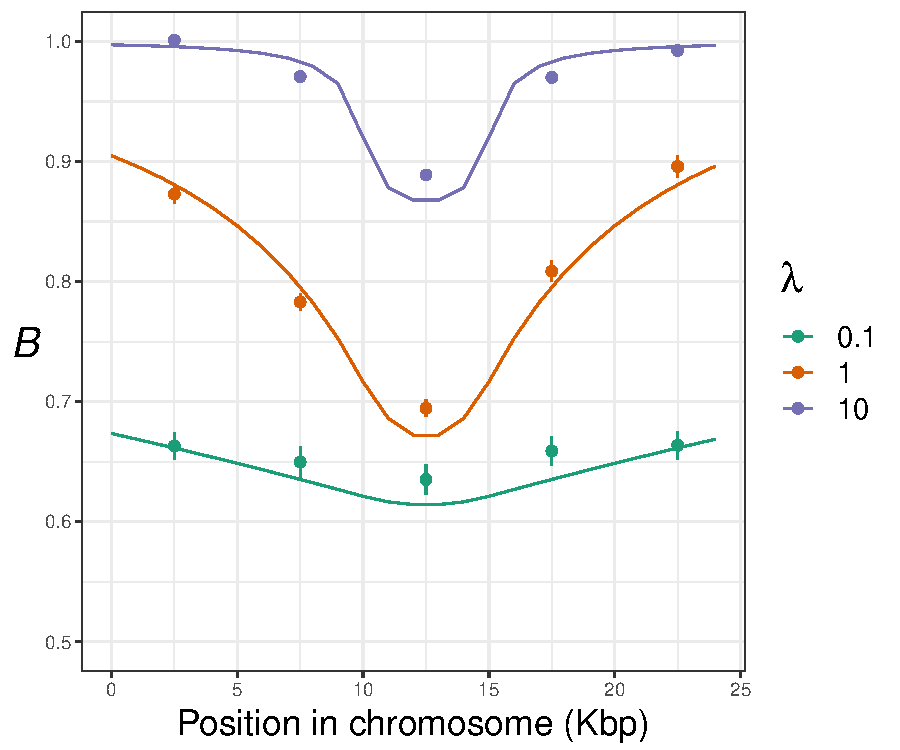
\includegraphics[width=0.7\textwidth]{../TheoreticalExpectation/B_fixed_plot}\centering
\caption{The effects of background selection across simulated chromosomes. \textit{B} was calculated for simulated data by comparing observed $\pi$ to the neutral expectation of $4N_e\mu=0.01$. The lines show the theoretical expectation calculated using formulae from Nordborg et al (1996).}
\label{fig:BGS_element_plot}
\end{figure}

\begin{figure}[h]
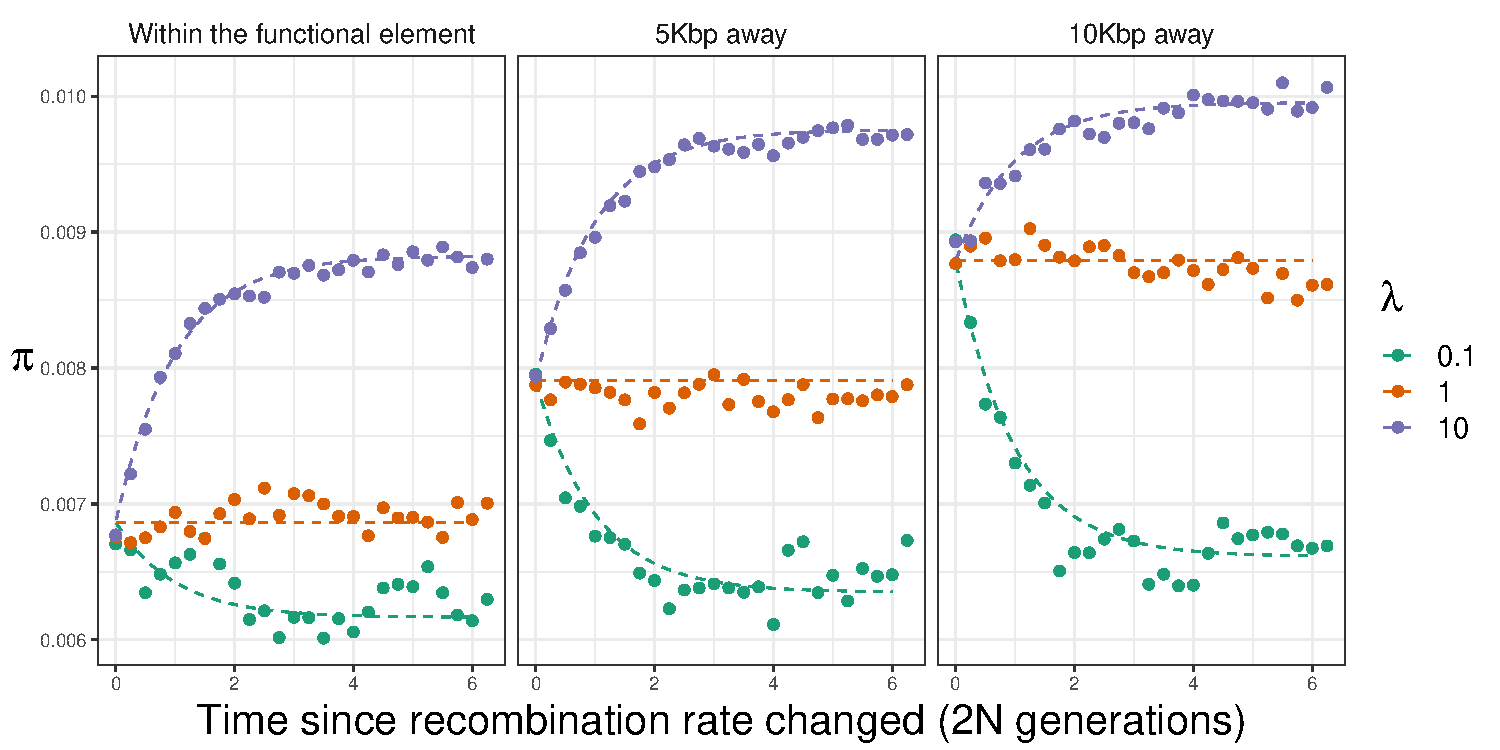
\includegraphics[width=\textwidth]{../TheoreticalExpectation/B_over_time_fixed_s_plot.pdf}
\caption{The effects of background selection across simulated chromosomes. \textit{B} was calculated for simulated data by comparing observed $\pi$ to the neutral expectation of $4N_e\mu=0.01$. The lines show the theoretical expectation calculated using formulae from Nordborg et al (1996). The labels on the top of each panel indicate the location in the simulated data being analysed.}
\label{fig:BGS_over_time_multiPanel}
\end{figure}


\begin{figure}[h]
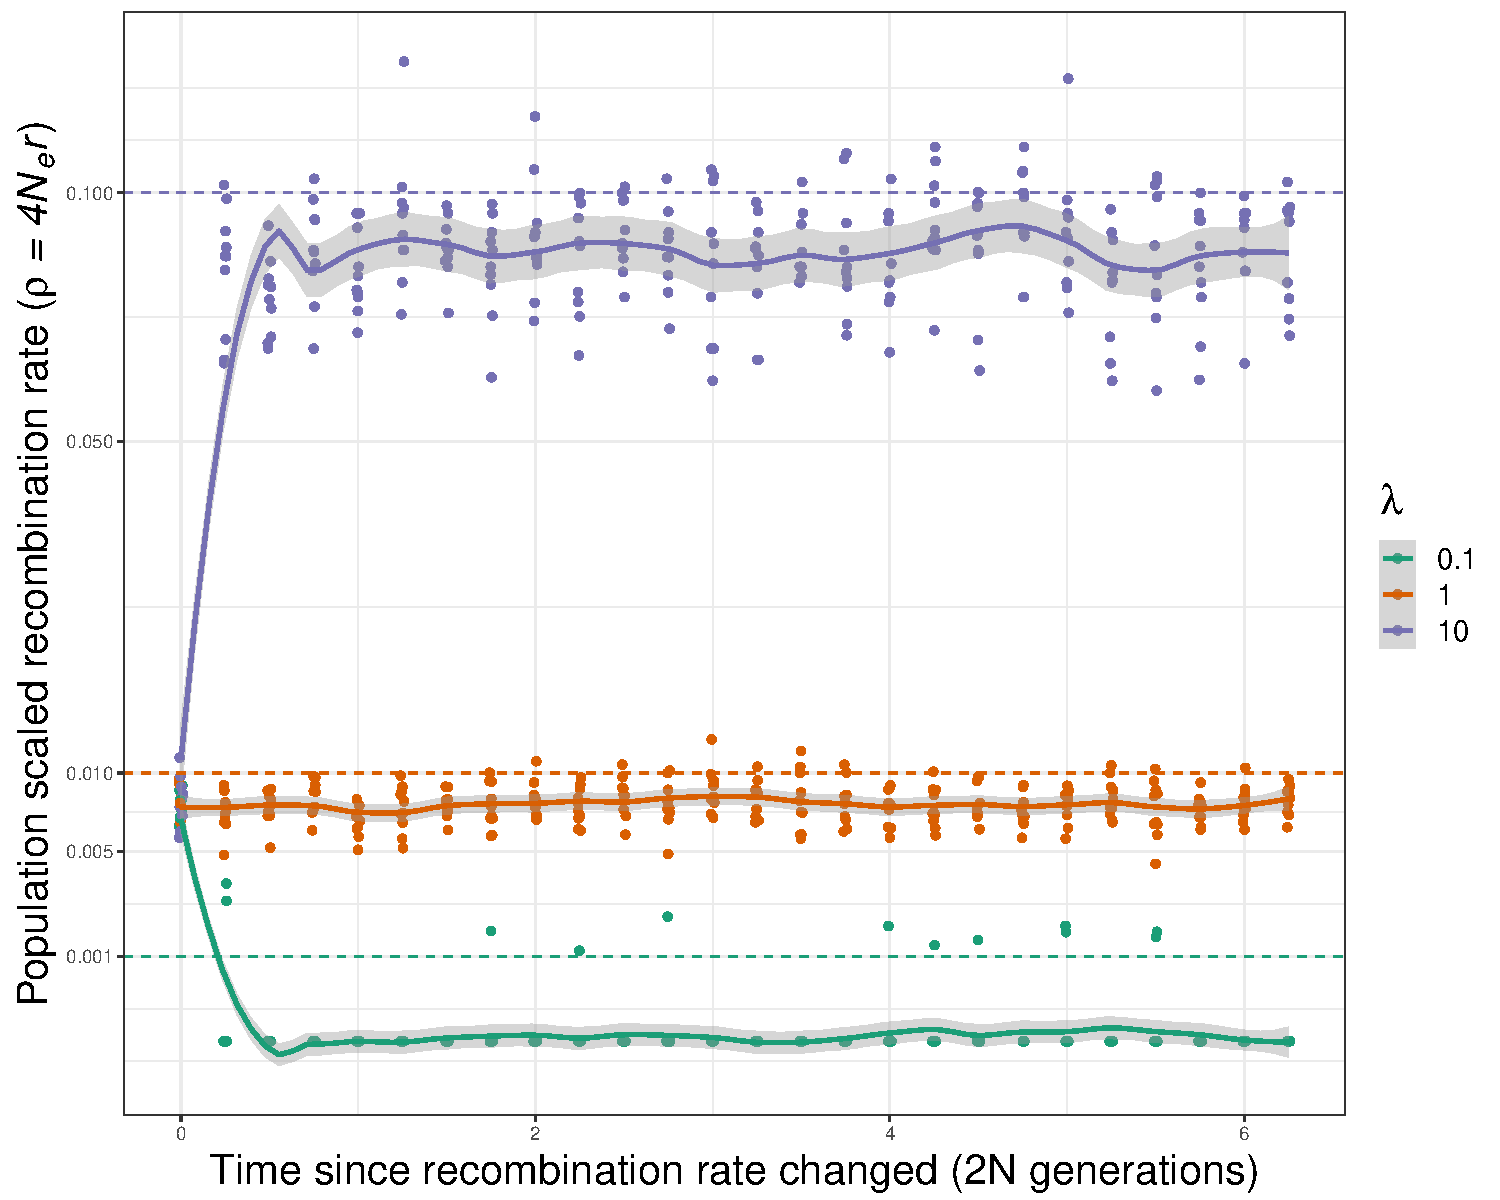
\includegraphics[width=\textwidth]{../TheoreticalExpectation/recRatesPlot.pdf}
\caption{Recombination rates inferred using \textit{PyRho} after an instantaneous change in the recombination rate. Dashed horizontal lines indicate the true recombination rate for the three cases. Smoothed lines with shaded ribbon indicate the fit and error of a LOESS regression.
}
\label{fig:recombinationRateEstimates}
\end{figure}


\begin{figure}[h]
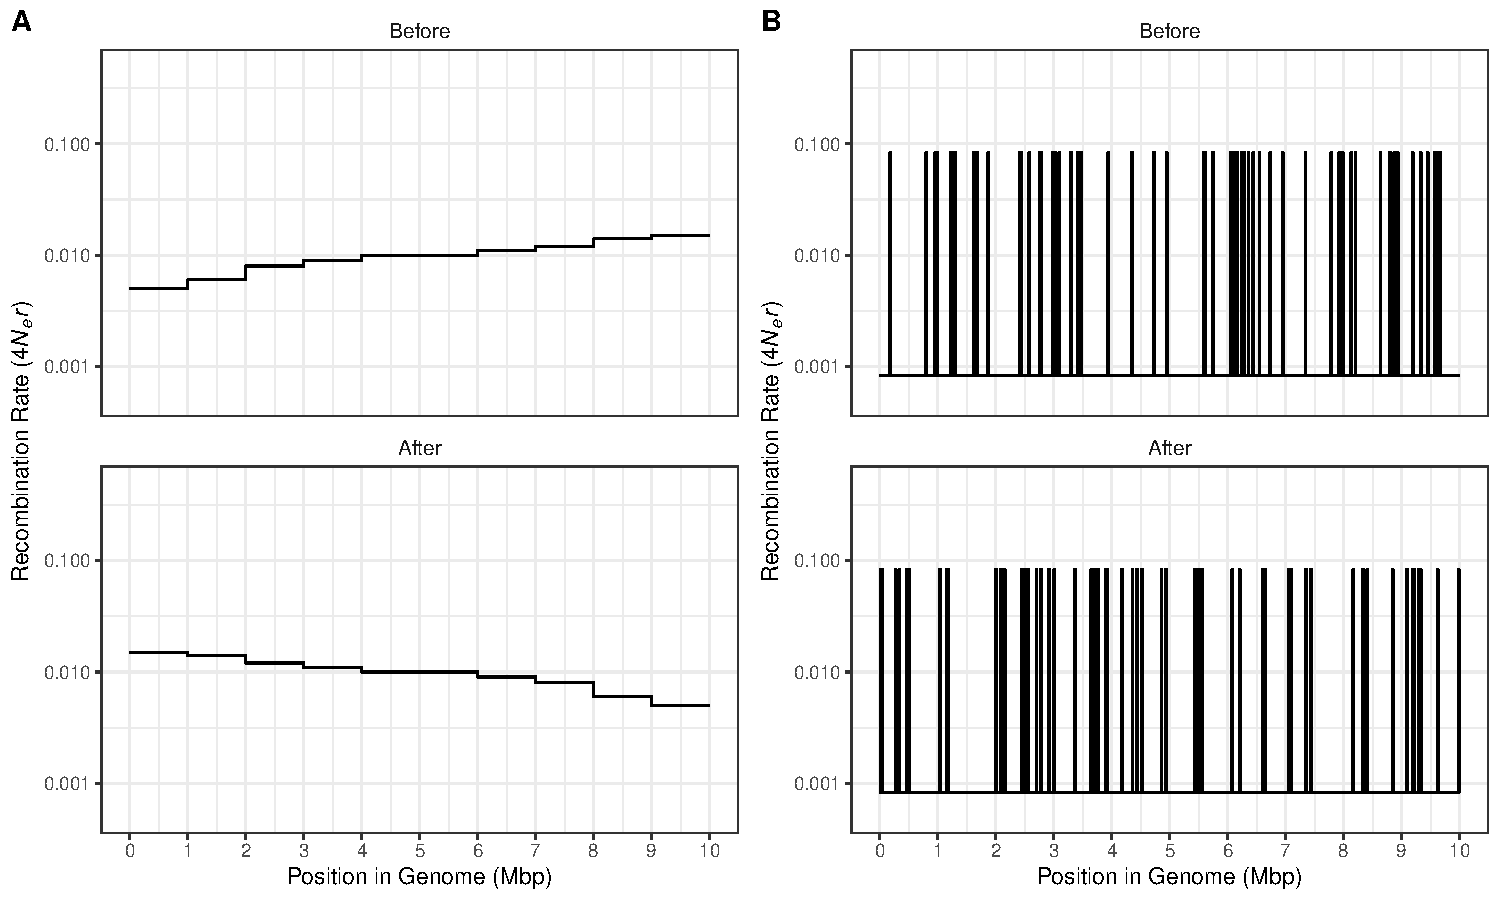
\includegraphics[width=\textwidth]{../Plots/recombinationMapDiagram.pdf}
\caption{The recombination rate maps used in the simulations modelling BGS across the genome. The upper and lower panels show the recombination rate landscape landscape before and after it evolved in simulations, repsectively. A) Evolution of the recombination rate at the Mbp scale. B) Evolution of the recombination rate at the scale of recombination hotspots.}
\label{fig:recombinationRateMaps}
\end{figure}



\begin{figure}[h]
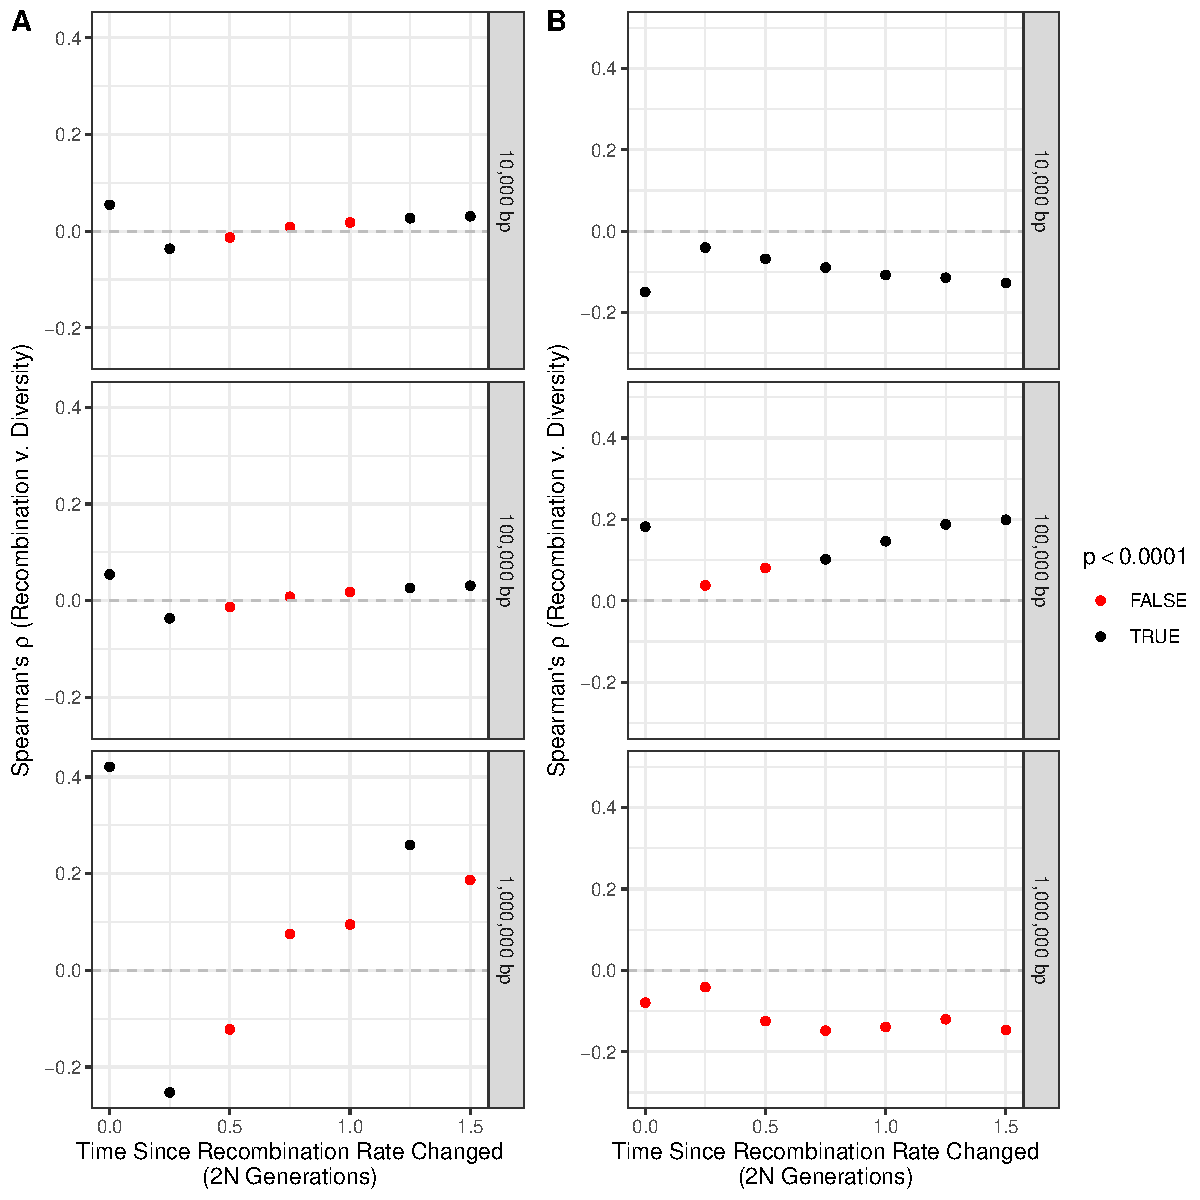
\includegraphics[width=\textwidth]{../Plots/pi_r_correlationOverTime_bothMaps_allWindows.pdf}
\caption{The correlation between nucleotide diversity and recombination rate over time after evolution of the recombination landscape. Panel A) shows results for the model of broadscale recombination rate evolution. Panel B) shows the results for the model of recombination hotspot evolution. In both the text in the grey strips to the right of each cell indicates the size of analysis windows used.}
\label{fig:recombinationRateMaps}
\end{figure}

\end{document}


The first empirical evidence that selection at linked sites influences genetic variation across the genome came from studies in \textit{Drosophila}. Aguadé et al (1989) measured genetic variability in the \textit{yellow-achaete-scute} regions located at the tip of the X-chromosome. The \textit{yellow-achaete-scute} regions experience restricted crossing-over and Aguadé et al (1989) found that they harbour far less genetic variation than had been reported for more highly recombining regions of the genome. Aguadé et al (1989) suggested that selective sweeps (though that term was not coined until later), which reduce nucleotide diversity ($\pi$) to the greatest extent in regions of restricted recombination, potentially explained their findings. Begun and Aquadro (1992) then showed that there is a clear correlation between recombination rate and nucleotide diversity ($\pi$) using loci sampled from across the \textit{D. melanogaster} genome. Furthermore, Begun and Aquadro (1992) showed that there was little evidence for a correlation of between-species divergence and recombination rate, which one might expect if recombination were itself mutagenic. Soon afterwards, Charlesworth et al (1993) demonstrated that background selection could also potentially explain the correlation between $\pi$ and the recombination rate.  \\